%***************************************************************************
%	PLANTILLA PARA LA EDICIÓN DE TRABAJOS FIN DE GRADO Y TESIS FIN DE MÁSTER
%	Departamento de Teoría de la Señal y Comunicaciones
%	Universidad de Alcalá
%***************************************************************************
%Fecha de última motificación: 28-Mayo-2021

%******************
%Tipo de documento
%******************
%Descomentar la opción que corresponda:
%Versión durante la revisión (incluye números de línea)
\documentclass[12pt,twoside,a4paper]{book}
%*****************************
%Paquetes que solemos utilizar
%*****************************

\usepackage[square,numbers]{natbib}
\usepackage[T1]{fontenc}
\usepackage[spanish]{babel}
\usepackage{verbatim}
\usepackage{amsmath}
\usepackage{acronym}
\usepackage{fancyhdr}
\usepackage{multicol}
\usepackage{makeidx}
\usepackage{float}
\usepackage[utf8]{inputenc}
\usepackage{color}
\usepackage{multirow}
\usepackage{url}
\usepackage{listings}
\lstset{language = Pascal}
\lstset{literate=
  {á}{{}}1 {é}{{Áé}}1 {í}{{í}}1 {ó}{{ó}}1 {ú}{{ú}}1
  {Á}{{Á}}1 {É}{{É}}1 {Í}{{Í}}1 {Ó}{{Ó}}1 {Ú}{{Ú}}1
  {à}{{à}}1 {è}{{è}}1 {ì}{{ì}}1 {ò}{{ò}}1 {ù}{{ù}}1
  {À}{{À}}1 {È}{{È}}1 {Ì}{{Ì}}1 {Ò}{{Ò}}1 {Ù}{{Ù}}1
  {ä}{{ä}}1 {ë}{{ë}}1 {ï}{{ï}}1 {ö}{{ö}}1 {ü}{{ü}}1
  {Ä}{{Ä}}1 {Ë}{{Ë}}1 {Ï}{{Ï}}1 {Ö}{{Ö}}1 {Ü}{{Ü}}1
  {â}{{â}}1 {ê}{{ê}}1 {î}{{î}}1 {ô}{{ô}}1 {û}{{û}}1
  {Â}{{Â}}1 {Ê}{{Ê}}1 {Î}{{Î}}1 {Ô}{{Ô}}1 {Û}{{Û}}1
  {ã}{{ã}}1 {ẽ}{{ẽ}}1 {ĩ}{{ĩ}}1 {õ}{{õ}}1 {ũ}{{ũ}}1
  {Ã}{{Ã}}1 {Ẽ}{{Ẽ}}1 {Ĩ}{{Ĩ}}1 {Õ}{{Õ}}1 {Ũ}{{Ũ}}1
  {œ}{{\oe}}1 {Œ}{{\OE}}1 {æ}{{\ae}}1 {Æ}{{\AE}}1 {ß}{{\ss}}1
  {ű}{{\H{u}}}1 {Ű}{{\H{U}}}1 {ő}{{\H{o}}}1 {Ő}{{\H{O}}}1
  {ç}{{ç}}1 {Ç}{{Ç}}1 {ø}{{\o}}1 {Ø}{{\O}}1 {å}{{\r a}}1 {Å}{{\r A}}1
  {€}{{\euro}}1 {£}{{\pounds}}1 {«}{{\guillemotleft}}1
  {»}{{\guillemotright}}1 {ñ}{{ñ}}1 {Ñ}{{Ñ}}1 {¿}{{?`}}1 {¡}{{!`}}1
}



% Esquemas de directorios y archivos
\usepackage[edges]{forest}
\definecolor{folderbg}{RGB}{124,166,198}
\definecolor{folderborder}{RGB}{110,144,169}
\newlength\Size
\setlength\Size{4pt}
\tikzset{%
  folder/.pic={%
    \filldraw [draw=folderborder, top color=folderbg!50, bottom color=folderbg] (-1.05*\Size,0.2\Size+5pt) rectangle ++(.75*\Size,-0.2\Size-5pt);
    \filldraw [draw=folderborder, top color=folderbg!50, bottom color=folderbg] (-1.15*\Size,-\Size) rectangle (1.15*\Size,\Size);
  },
  file/.pic={%
    \filldraw [draw=folderborder, top color=folderbg!5, bottom color=folderbg!10] (-\Size,.4*\Size+5pt) coordinate (a) |- (\Size,-1.2*\Size) coordinate (b) -- ++(0,1.6*\Size) coordinate (c) -- ++(-5pt,5pt) coordinate (d) -- cycle (d) |- (c) ;
  },
}
\forestset{%
  declare autowrapped toks={pic me}{},
  pic dir tree/.style={%
    for tree={%
      folder,
      font=\ttfamily,
      grow'=0,
    },
    before typesetting nodes={%
      for tree={%
        edge label+/.option={pic me},
      },
    },
  },
  pic me set/.code n args=2{%
    \forestset{%
      #1/.style={%
        inner xsep=2\Size,
        pic me={pic {#2}},
      }
    }
  },
  pic me set={directory}{folder},
  pic me set={file}{file},
}

% -------- Nuevos paquetes -------

\usepackage{siunitx}
\usepackage{pdflscape}
\usepackage[newfloat]{minted}
\usepackage{caption}
\usepackage[dvipsnames]{xcolor}
\usepackage{tikz}
\usepackage[pages=some]{background}
\usepackage{appendix}
\usepackage{comment}
\usepackage{graphicx}
\usepackage{subcaption}
\usepackage{colortbl}
\usepackage{matlab-prettifier}
\usepackage{eurosym}
%\usepackage{utils/symbols}


\newenvironment{code}{\captionsetup{type=listing}}{}
\SetupFloatingEnvironment{listing}{name=Código Fuente}
% --------------------------------

\makeatletter
\expandafter\let\csname active@char\string?\endcsname\relax
\expandafter\let\csname active@char\string!\endcsname\relax
\expandafter\let\csname active@char\string:\endcsname\relax


\initiate@active@char{?}
\initiate@active@char{!}
\initiate@active@char{:}
\makeatother
%No incluir paquetes depués de este.

%*************
%Definiciones
%*************
\deactivatetilden
\addto\captionsspanish{\def\tablename{Tabla}\def\listtablename{Lista
de tablas}\def\listfigurename{Lista de figuras}}
%Cambios en los márgenes
\renewcommand{\baselinestretch}{1.1}

\setlength{\oddsidemargin}{0.4cm}
\setlength{\evensidemargin}{-0.4cm} \setlength{\headsep}{0.75cm}
\setlength{\textheight}{23cm} \setlength{\textwidth}{16cm}
\setlength{\topmargin}{-0.25cm}\flushbottom



%***************
%Título del trabajo
%***************
\title{Desarrollo de soluciones para navegación robótica basadas en segmentación semántica y aprendizaje por imitación.}

%****************
%Autor
%****************
\author{Rafael Flor Rodríguez-Rabadán}

%Prepara el índice
\makeindex



%***********************
%Comienzo del documento
%***********************
\begin{document}
\setcounter{tocdepth}{4} \setcounter{secnumdepth}{3}

\frontmatter

%Incluimos fichero previo.tex -> genera la hoja de calificación y la portada
\begin{titlepage}
%**********************************************************
%GENERA LA HOJA OFICIAL DE CALIFICACIÓN 
%SEGÚN EL FORMATO DE LA NORMATIVA DE LA EPS UAH
%**********************************************************


\begin{center}
%Incluye logo de la UAH


\includegraphics[width=15cm]{figuras/logo-uah.pdf}\\
\vspace{0.5cm}


\LARGE  \textbf{Escuela Politécnica Superior}\\


%Titulación -> escriba su titulación
Máster Universitario en Ingeniería de Telecomunicación\\
\end{center}

\vspace{0.5cm}



\begin{center}
\vspace{0.5cm}

%Seleccione el que corresponda
%\LARGE Trabajo Fin de Grado\\
\LARGE Tesis Fin de Máster\\

\textbf{\Huge \textsc{{Desarrollo de soluciones para navegación robótica basadas en segmentación semántica y aprendizaje por imitación.}}}\\
\vspace{0.5cm}
\large Autor: Rafael Flor Rodríguez-Rabadán.\\
Tutor: Roberto Javier López Sastre.\\
Cotutor: Carlos Gutiérrez Álvarez.\\
\vspace{0.5cm}
\end{center}

\begin{flushleft}
\textbf{TRIBUNAL:}\\
\vspace{1cm}
\textit{Presidente: D. Nombre y apellidos del presidente}\\
\vspace{1cm}
\textit{Vocal 1º: D. Nombre y apellidos del vocal 1}\\
\vspace{1cm}
\textit{Vocal 2º: D. Nombre y apellidos del vocal 2}\\
\vspace{1cm}
\textbf{FECHA:} indicar la fecha de depósito\\ 

\end{flushleft}
%Final de la hoja de calificación.

%Introduce hoja en blanco
\newpage
\thispagestyle{empty}
\hspace*{0.5cm}
\newpage


\end{titlepage}

%Prepara el título del proyecto.
\maketitle

%Introduce hoja en blanco
\newpage
\thispagestyle{empty}
\hspace*{0.5cm}
\newpage

%Incluye las dedicatorias (fichero dedicatorias.tex)
\begin{flushright}
\textit{Aquí escribes las dedicatorias. Por ejemplo: A mis padres.}
\end{flushright}
%Introduce hoja en blanco
\newpage
\thispagestyle{empty}
\hspace*{0.5cm}
\newpage


%Incluye los agradecimientos (fichero agradecimientos.tex)
\chapter{Agradecimientos}
Aquí debes incluir los agradecimientos.

%Introduce hoja en blanco
\newpage
\thispagestyle{empty}
\hspace*{0.5cm}
\newpage


%Inlcuimos el índice que latex genera automáticamente.
\tableofcontents
%La lista de figuras incluidas en el proyecto.
\listoffigures
%La lista de tablas.
\listoftables


%Incluye el resumen del Proyecto fin de carrera (fichero resumen.tex)
\chapter{Resumen}
\textcolor{red}{Resumen de 100 palabras MÁXIMO}\\

\vspace{0.5cm}

\textbf{Palabras clave}: cinco palabras como máximo, separadas por comas.

%Introduce hoja en blanco
\newpage
\thispagestyle{empty}
\hspace*{0.5cm}
\newpage

\chapter{Abstract}
\textcolor{red}{Resumen de 100 palabras MÁXIMO - Es OBLIGATORIO}\\

\vspace{0.5cm}

\textbf{Keywords}: cinco palabras como máximo, separadas por comas.
%Introduce hoja en blanco
\newpage
\thispagestyle{empty}
\hspace*{0.5cm}
\newpage

%Incluye el resumen Extendido del Proyecto fin de carrera (fichero resumen-extendido.tex)
\chapter{Resumen Extendido}
Debe incluir un resumen del trabajo de un máximo de 5 páginas. Resaltar aspectos fundamentales del desarrollo, los resultados más relevantes y las conclusiones.



%Incluimos lista de abreviaturas
\chapter{Glosario}

%Lista con los acrónimos
\begin{acronym}[PFC]
\item \acro{TFG}{Trabajo fin de Grado}
\item \acro{TFM}{Tesis fin de Máster}
\end{acronym}

%Para poner más acrónimos
%\acro{ACRÓNIMO}{Descripción del acrónimo}







\mainmatter

%Incluimos los capítulos del proyecto. Cada capitulo se encuentra en un fichero tex,
%que insertamos en el documento por medio del comando \include{capitulo-cualquiera}

%Incluye Introducción (fichero introduccion.tex)
\chapter{Introducción}\label{ch:introduccion}

La habilidad del ser humano para navegar en entornos desconocidos se fundamenta en su capacidad para identificar patrones comunes entre diversas estancias.
Esto le permite, mediante un proceso de exploración, localizar su objetivo en un espacio nunca antes visitado.

Esta capacidad para recorrer entornos desconocidos ha demostrado ser de gran interés para su integración en plataformas robóticas reales, debido a su versatilidad tanto funcional como comercial.
Históricamente, en el ámbito de la robótica, la navegación ha estado estrechamente vinculada a la sensorización y al uso de tecnologías como \ac{LiDAR}, empleando técnicas como \ac{SLAM}.
No obstante, estas aproximaciones presentan limitaciones a la hora de generalizar el problema de la navegación en entornos no explorados, además de mayores desafíos en escenarios abiertos o simétricos.

Como alternativa, actualmente se aborda este reto mediante el uso de redes neuronales entrenadas con diversos algoritmos de \textit{Deep Learning}.
Es lo que se conoce como las soluciones de navegación basadas en aprendizaje, que emplean, principalmente, sensores visuales.
Es por ello, que el problema recibe el nombre de Navegación Visual Semántica.
Algunos de los trabajos más recientes en esta dirección son los siguientes\citep{ramrakhya2023,zhang2022,Huang2023}.

El entrenamiento de estas soluciones se lleva a cabo en entornos virtuales, donde un agente tiene la capacidad de desplazarse por espacios reales renderizados.
Esta metodología permite acelerar el proceso de aprendizaje al aprovechar máquinas especializadas en computación paralela, y algoritmos diversos como el aprendizaje por refuerzo o el aprendizaje por imitación.

Con el fin de demostrar y comparar la capacidad de navegación de estos agentes, se les asigna la tarea de localizar un objeto dentro de estancias renderizadas, las cuales no han explorado previamente.

Se ha demostrado que estos agentes son capaces de alcanzar altos porcentajes de éxito en la consecución de sus objetivos dentro de entornos virtuales.
No obstante, cuando se implementan estas redes en el mundo real, surgen desafíos relacionados con la \textit{\textbf{adaptación de dominio}}.
Estos problemas se deben, en parte, a la menor precisión de los sensores y a factores inherentes al entorno físico, como variaciones en la iluminación.

El propósito de estas redes neuronales es emular el comportamiento humano, lo cual explica que las entradas a las redes correspondan habitualmente a los mismos estímulos sensoriales que utilizan los seres humanos.
Por esta razón, se emplean de manera predominante imágenes RGB, odometría y cámaras de profundidad.
Sin embargo, el ser humano no se desplaza únicamente en función de las imágenes que percibe, sino que también otorga un sentido semántico a los objetos dentro de esas imágenes.
De este modo, es capaz de identificar rápidamente la función de cada elemento que observa, como suelos, paredes, armarios o sillas, asignándoles una categoría semántica de manera casi instantánea.

Esta capacidad para categorizar visualmente ha sido abordada con gran éxito en el campo de la visión artificial.
En la actualidad, contamos con segmentadores semánticos que han demostrado un rendimiento sobresaliente\cite{Seichter2020EfficientRS}.

En este proyecto, pretendemos estudiar el impacto que los sensores de segmentación semántica tienen en los modelos de navegación visual semántica.
Postulamos que son una fuente de información que puede aliviar el problema de la adaptación de dominio, y, por lo tanto, el desarrollo de modelos de navegación que puedan funcionar en el mundo real, y no solo en entornos virtuales.

Así, en este trabajo, proponemos desarrollar soluciones de navegación visual semántica empleando aprendizaje por imitación (\textbf{IL} (Imitation Learning)) que recibirán imágenes de segmentación semántica como entrada.
Posteriormente, se comparará su rendimiento con respecto a modelos que utilizan imágenes RGB, tanto en entornos virtuales como en escenarios del mundo real.

En la figura\ref{fig:semnav} proponemos una representación del tipo de soluciones que se van a desarrollar, denominadas como SemNav, puede observarse como a la entrada de la red se ingresará información de segmentación semántica, complementada con otro tipo de información, que ayudará al modelo a completar la navegación en entornos desconocidos.

\begin{figure}
    \centering
    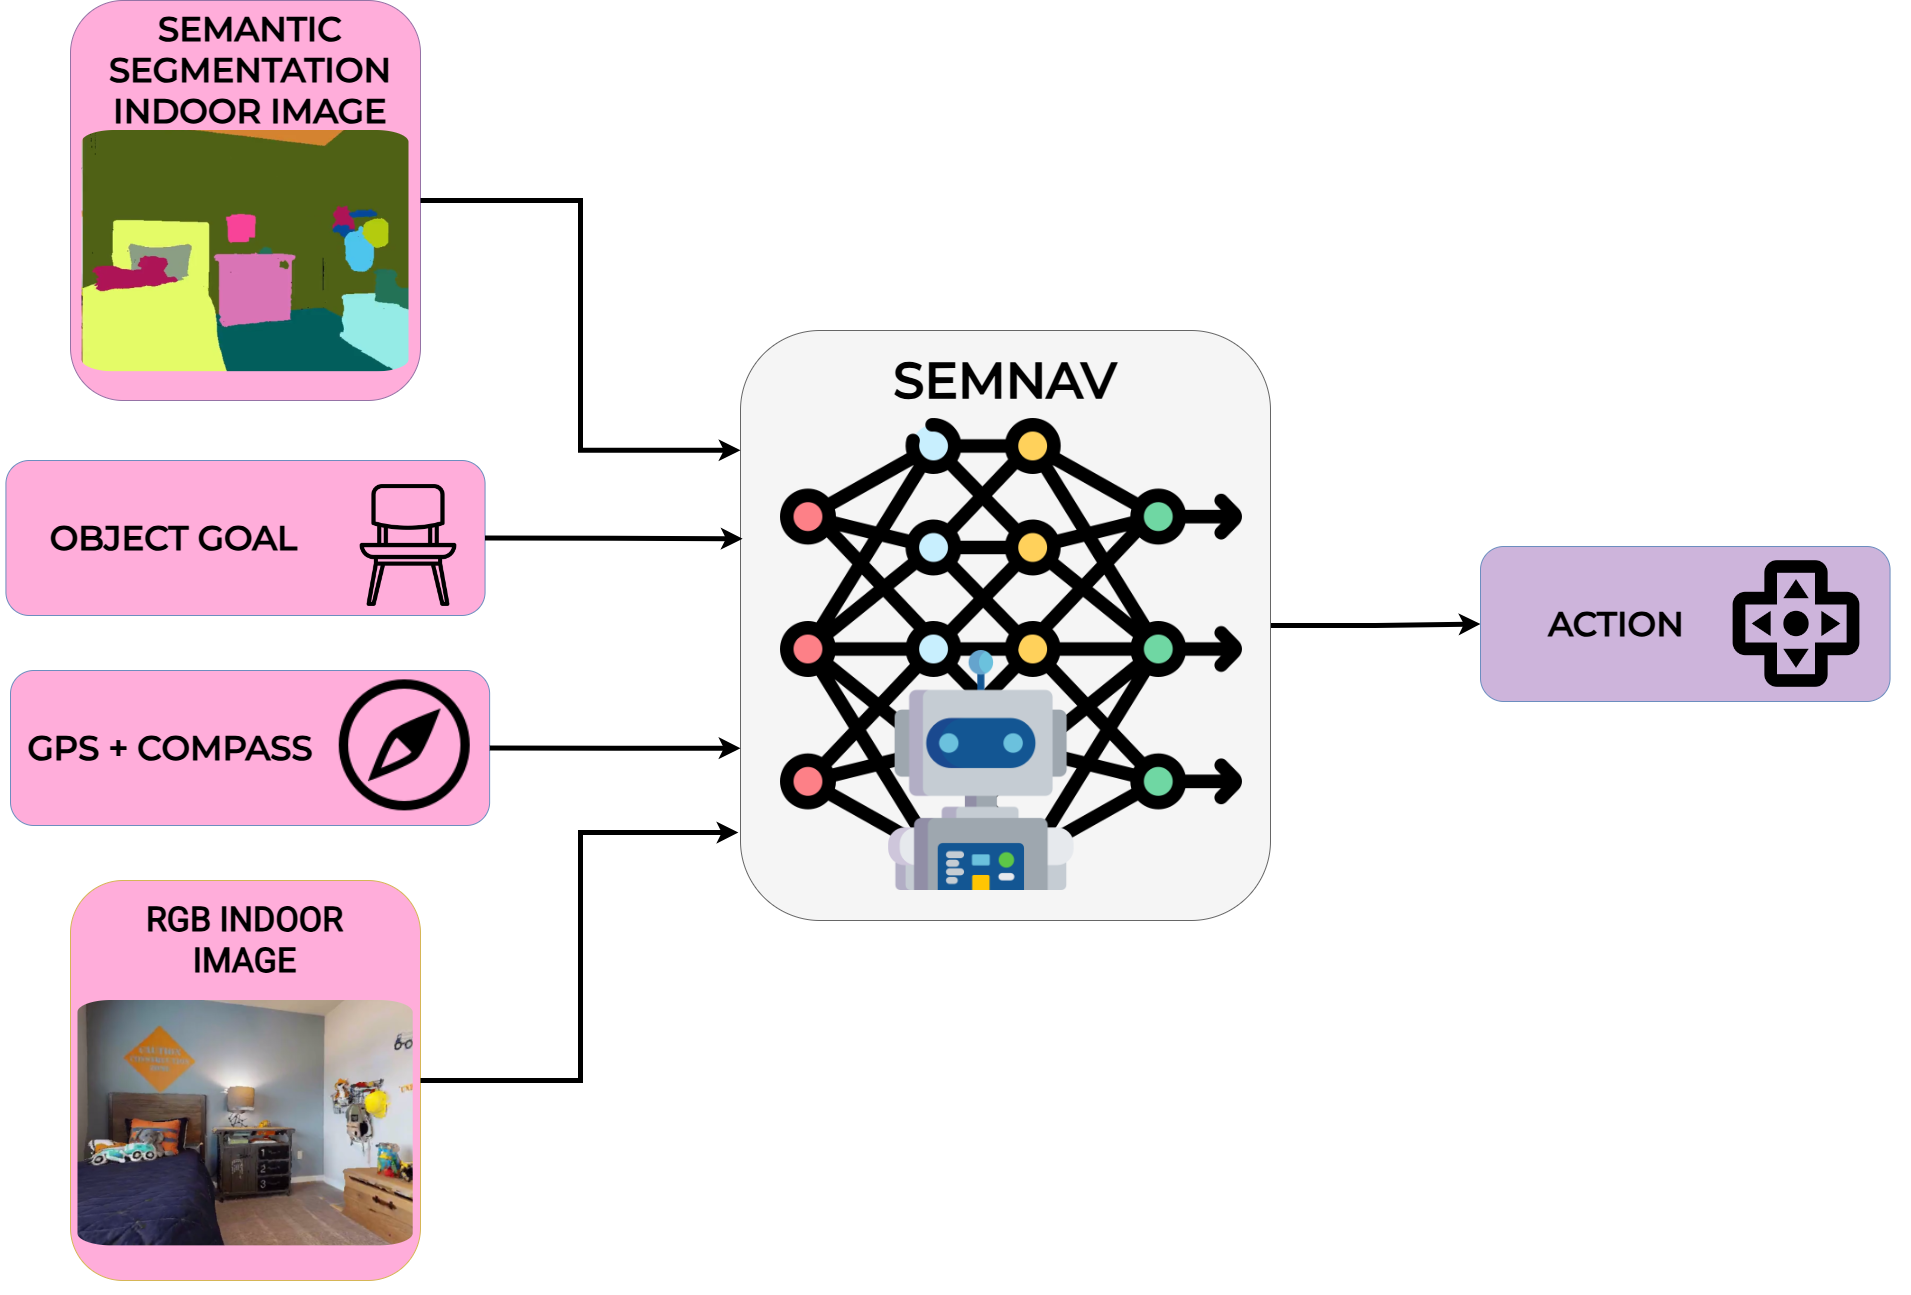
\includegraphics[width=\textwidth]{figuras/semnav_model}
    \caption{Modelo SEMNav para la navegación basada en información de segmentación semántica del entorno.}
    \label{fig:semnav}
\end{figure}
\chapter{Desarrollo del modelo y dataset para la navegación mediante segmentación semántica}\label{ch:desarrollo-del-modelo-y-dataset-para-la-navegacion-mediante-segmentacion-semantica}

Como ya ha sido tratado en los capítulos anteriores de este documento, el modelo propuesto de navegación mediante segmentación semántica estará basado en el modelo propuesto por \texttt{PirlNav}\citep{ramrakhya2023} con las modificaciones indicadas en la figura



\begin{equation}
  floor(\frac{255*255*255}{num\_categories})\label{eq:constant}
\end{equation}
\begin{figure}
    \centering
    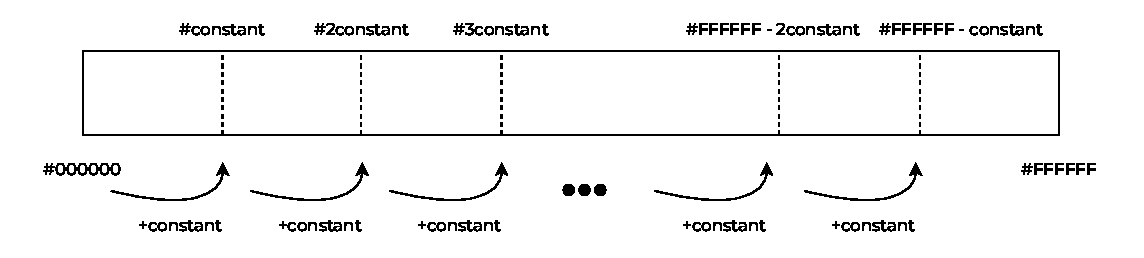
\includegraphics[width=\textwidth]{figuras/colored_scheme.drawio}
    \caption{Esquema de generación de colores mediante la suma de la constante producida por la ecuación\ref{eq:constant}.}
    \label{fig:constant_scheme}
\end{figure}
\begin{figure}
    \centering
    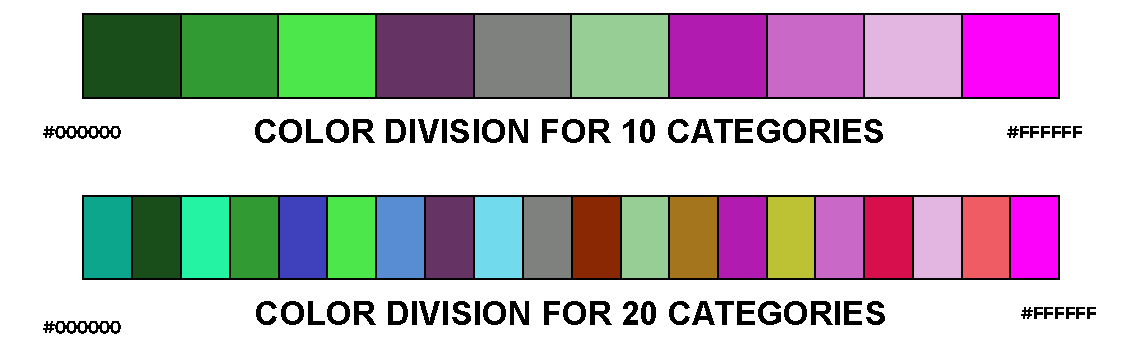
\includegraphics[width=\textwidth]{figuras/morecolored_scheme.drawio}
    \caption{ Ejemplo de generación de colores mediante la estrategia de suma de constante para 10 y 20 categorías.}
    \label{fig:colored_scheme}
\end{figure}
\begin{figure}
    \centering
    \includegraphics[width=0.4\textwidth]{images/vertical_color_gradient_640x480}
    \caption{ Fotografía generada mediante estrategia de división del espectro del color.}
    \label{fig:colorinchis}
\end{figure}
\section{Resultados}

% Please add the following required packages to your document preamble:
% \usepackage{multirow}
\definecolor{lightblue}{RGB}{173, 216, 230}

\begin{table}[H]
\begin{tabular}{l|cccccc|}
\cline{2-7}
                                               & \multicolumn{6}{c|}{\textbf{SR}}                                                                                                                                                                  \\ \cline{2-7}
\textbf{}                                      & \multicolumn{2}{c|}{\textbf{SEMANTIC + RGB}}                & \multicolumn{2}{c|}{\textbf{ONLY SEMANTIC}}              & \multicolumn{2}{c|}{\textbf{PIRLNAV}}                                    \\ \cline{2-7}
                                               & \multicolumn{1}{c|}{DINO}    & \multicolumn{1}{c|}{NO DINO} & \multicolumn{1}{c|}{DINO} & \multicolumn{1}{c|}{NO DINO} & \multicolumn{1}{l|}{DINO}                 & \multicolumn{1}{l|}{NO DINO} \\ \hline
\multicolumn{1}{|c|}{\textbf{1630 cat}} & \multicolumn{1}{c|}{70.0\%}  & \multicolumn{1}{c|}{69.2\%}  & \multicolumn{1}{c|}{I.P(14daysstopped)}     & \multicolumn{1}{c|}{65.1\%}  & \multicolumn{1}{c|}{\multirow{2}{*}{60.8\%}} & \multirow{2}{*}{39.5\%}         \\ \cline{1-5}
\multicolumn{1}{|c|}{\textbf{40 cat}}   & \multicolumn{1}{c|}{\cellcolor{lightblue}74.95\%} & \multicolumn{1}{c|}{74.3\%} & \multicolumn{1}{c|}{72.3\%}     & \multicolumn{1}{c|}{72.9\%}        & \multicolumn{1}{c|}{}                     &                              \\ \hline
\end{tabular}
\end{table}


\backmatter


%*****************************
%Sección para la bibliografía
%*****************************

%Posibles estilos de bibliografia
\bibliographystyle{plain}
%\bibliographystyle{abbrvnat}
%\bibliographystyle{klunamed}
%\bibliographystyle{unsrt}

\addcontentsline{toc}{chapter}{{}Bibliografía}

%Toma los datos del fichero bibliografia-proyecto.bib
\bibliography{bibliografia-proyecto}

%\printindex

\end{document}

%Final de la plantilla.
